% ------------------------------------------------------------------------------
% TYPO3 CMS 7.0 - What's New - Chapter "Deprecated Functions" (German Version)
%
% @author	Patrick Lobacher <patrick@lobacher.de>
% @license	Creative Commons BY-NC-SA 3.0
% @link		http://typo3.org/download/release-notes/whats-new/
% @language	German
% ------------------------------------------------------------------------------
% LTXE-CHAPTER-UID:		08661c9e-3f5aee5c-0b8f8af6-9681f2f1
% LTXE-CHAPTER-NAME:	Deprecated Functions
% ------------------------------------------------------------------------------
% LTXE-SLIDE-START
% LTXE-SLIDE-UID:		9471fc84-1a774dda-7d47ae2f-f1306fd8
% LTXE-SLIDE-ORIGIN:	xxxxxxxx-xxxxxxxx-xxxxxxxx-xxxxxxxx
% LTXE-SLIDE-TITLE:		Compatibility Layer
% LTXE-SLIDE-REFERENCE:	http://typo3.org/news/article/retaining-compatibility-to-typo3-cms6/
% ------------------------------------------------------------------------------

\begin{frame}[fragile]
	\frametitle{Veraltete/Entfernte Funktionen}
	\framesubtitle{Kompatibilitäts-Schicht}

	\begin{itemize}

		\item In TYPO3 CMS 6.2 stellt eine Kompatibilitäts-Schicht sicher,
			dass auch alte Extensions mit der neuen Codebase funktionieren\newline
			\small
				Nachteil: Geschwindigkeitseinbuße (das volle Potential des Systems kann nicht ausgeschöpft werden)
			\normalsize

		\item Diese Kompatibilitäts-Schicht wurde in TYPO3 CMS 7.0 entfernt\newline
			\small
				Auswirkung: alte Extensions sind möglicherweise nicht mehr lauffähig\newline(z.B. Extensions ohne Namespaces)
			\normalsize

		\item Kompatibilität kann aber wieder hergestellt werden, indem die System Extension \texttt{EXT:compatibility6} installiert wird
		\item Diese Extension wird zukünftig im TER verfügbar sein

	\end{itemize}

\end{frame}

% ------------------------------------------------------------------------------
% LTXE-SLIDE-START
% LTXE-SLIDE-UID:		5eefd123-43bfb1ca-1e9bc2a8-c3f26a33
% LTXE-SLIDE-ORIGIN:	xxxxxxxx-xxxxxxxx-xxxxxxxx-xxxxxxxx
% LTXE-SLIDE-TITLE:		Backend Benutzerverwaltung
% ------------------------------------------------------------------------------

\begin{frame}[fragile]
	\frametitle{Veraltete/Entfernte Funktionen}
	\framesubtitle{Backend Benutzerverwaltung}

	\begin{itemize}
		\item Funktion "zum Benutzer wechseln" \textit{(change-to mode)} wurde entfernt
	\end{itemize}

	\smaller\tabto{1cm}\begingroup\color{typo3red}TYPO3 CMS 6.2\endgroup\normalsize
	\begin{figure}\vspace{-0.4cm}
		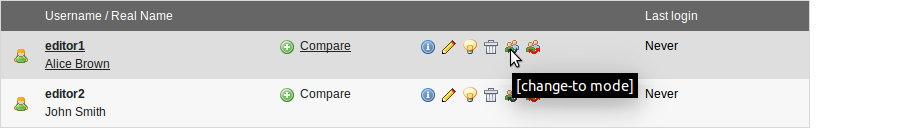
\includegraphics[width=0.90\linewidth]{DeprecatedRemovedFunctions/BackendUserSwitch1.png}
	\end{figure}

	\smaller\tabto{1cm}\begingroup\color{typo3red}TYPO3 CMS 7.0\endgroup\normalsize
	\begin{figure}\vspace{-0.4cm}
		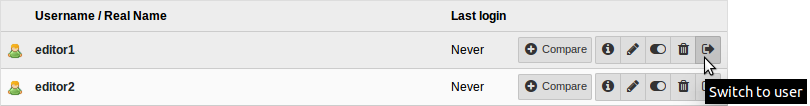
\includegraphics[width=0.90\linewidth]{DeprecatedRemovedFunctions/BackendUserSwitch2.png}
	\end{figure}

\end{frame}

% ------------------------------------------------------------------------------
% LTXE-SLIDE-START
% LTXE-SLIDE-UID:		8114d831-b4140a2c-e5c0122f-8112f75f
% LTXE-SLIDE-ORIGIN:	xxxxxxxx-xxxxxxxx-xxxxxxxx-xxxxxxxx
% LTXE-SLIDE-TITLE:		Veraltete JavaScript Funktionen entfernt
% LTXE-SLIDE-REFERENCE:	https://github.com/TYPO3/TYPO3.CMS/commit/2dff81b963e1b77c7f068f91ffde73914a18b0be
% LTXE-SLIDE-REFERENCE:	https://forge.typo3.org/issues/62291
% LTXE-SLIDE-REFERENCE:	https://forge.typo3.org/projects/typo3cms-core/repository/revisions/9ac03e383e4786e868f4b1d81893e84c4621abc8/entry/typo3/sysext/core/Documentation/Changelog/master/Breaking-62291-RTEDeprecatedJavaScriptMethodsRemoved.rst
% ------------------------------------------------------------------------------

\begin{frame}[fragile]
	\frametitle{Veraltete/Entfernte Funktionen}
	\framesubtitle{Veraltete JavaScript Funktionen entfernt}

	\begin{itemize}
		\item In Einklang mit der \href{http://forge.typo3.org/projects/typo3v4-core/wiki/CoreDevPolicy}{Deprecation Strategy}
			wurden in TYPO3 CMS 4.7 zahlreiche JavaScript Methoden als \textit{deprecated} markiert und nun entfernt, beispielsweise:

		\begin{lstlisting}
			\TYPO3\CMS\Backend\Form\FormEngine->getSingleField_typeInput
			\TYPO3\CMS\Backend\Form\FormEngine->getSingleField_typeText
			\TYPO3\CMS\Core\Utility\GeneralUtility->quoted_printable
			\TYPO3\CMS\Core\Utility\GeneralUtility->encodeHeader
		\end{lstlisting}

		\smaller
			\texttt{HTMLArea.Editor.forceRedraw}\newline
				(use \texttt{HTMLArea.Framework.doLayout} instead)
				\vspace{0.2cm}

			\texttt{HTMLArea.Editor.convertNode}\newline
				(use \texttt{HTMLArea.DOM.convertNode} instead)
				\vspace{0.2cm}

			\texttt{HTMLArea.Editor.getBlockAncestors}\newline
				(use \texttt{HTMLArea.DOM.getBlockAncestors} instead)
		\normalsize

	\end{itemize}

\end{frame}

% ------------------------------------------------------------------------------
% LTXE-SLIDE-START
% LTXE-SLIDE-UID:		ac3f9c77-e1a32beb-fd80e940-fb5dd699
% LTXE-SLIDE-ORIGIN:	xxxxxxxx-xxxxxxxx-xxxxxxxx-xxxxxxxx
% LTXE-SLIDE-TITLE:		Entfernte Funktionen (1)
% LTXE-SLIDE-REFERENCE:	https://forge.typo3.org/issues/17579
% LTXE-SLIDE-REFERENCE:	https://forge.typo3.org/issues/62888
% ------------------------------------------------------------------------------

\begin{frame}[fragile]
	\frametitle{Veraltete/Entfernte Funktionen}
	\framesubtitle{Entfernte Funktionen (1)}

	\begin{itemize}

		\item
			\small
				TypoScript Option \texttt{config.uniqueLinkVars} wurde entfernt\newline
				(das ist nun das Standardverhalten in TYPO3 CMS)
			\normalsize

		\item
			\small
				ViewHelper
					\texttt{\textbackslash
						TYPO3\textbackslash
						CMS\textbackslash
						Documentation\textbackslash
						ViewHelpers\textbackslash
						Link\textbackslash
						Action}
					wurde entfernt (benutze \texttt{f:be.buttons.icon} or \texttt{f:uri.*} stattdessen)
			\normalsize

		\item
			\small
				PageTSconfig Option \texttt{mod.web\_list.alternateBgColors}\newline
				wurde entfernt
			\normalsize

		\item
			\small
				PropertyMapper wurde entfernt\newline
				(ebenso die Option \texttt{rewrittenPropertyMapper = 0})
			\normalsize

		\item
			\small
				Folgende TypoScript Conditions wurden entfernt:

					\begin{itemize}
						\item\texttt{browser}
						\item\texttt{version}
						\item\texttt{system}
						\item\texttt{useragent}
					\end{itemize}
			\normalsize

	\end{itemize}

\end{frame}

% ------------------------------------------------------------------------------
% LTXE-SLIDE-START
% LTXE-SLIDE-UID:		46f3093f-809a8710-4ddb7317-cc5c4e1e
% LTXE-SLIDE-ORIGIN:	xxxxxxxx-xxxxxxxx-xxxxxxxx-xxxxxxxx
% LTXE-SLIDE-TITLE:		Entfernte Methoden (1)
% ------------------------------------------------------------------------------

\begin{frame}[fragile]
	\frametitle{Veraltete/Entfernte Funktionen}
	\framesubtitle{Entfernte Methoden (1)}

	Die folgenden \textbf{Methoden} wurden entfernt:

	\begin{itemize}
		\item
			\small
				\texttt{connectDB}\newline
				in der Klasse
				\texttt{\textbackslash
					TYPO3\textbackslash
					CMS\textbackslash
					Frontend\textbackslash
					Utility\textbackslash
					EidUtility}
			\normalsize
		\item
			\small
				\texttt{isDisplayCondition}\newline
				in der Klasse
				\texttt{\textbackslash
					TYPO3\textbackslash
					CMS\textbackslash
					Form\textbackslash
					FormEngine}
			\normalsize
		\item
			\small
				\texttt{int\_from\_ver}\newline
				in der Klasse
				\texttt{\textbackslash
					TYPO3\textbackslash
					CMS\textbackslash
					Core\textbackslash
					Utility\textbackslash
					GeneralUtility}
			\normalsize
		\item
			\small
				\texttt{getUniqueFields}\newline
				in der Klasse
				\texttt{\textbackslash
					TYPO3\textbackslash
					CMS\textbackslash
					Core\textbackslash
					DataHandling\textbackslash
					DataHandler}
			\normalsize

	\end{itemize}

\end{frame}


% ------------------------------------------------------------------------------
% LTXE-SLIDE-START
% LTXE-SLIDE-UID:		09be6038-7a3c9b4a-7783cf40-247898e9
% LTXE-SLIDE-ORIGIN:	xxxxxxxx-xxxxxxxx-xxxxxxxx-xxxxxxxx
% LTXE-SLIDE-TITLE:		Entfernte Methods (2)
% ------------------------------------------------------------------------------

\begin{frame}[fragile]
	\frametitle{Veraltete/Entfernte Funktionen}
	\framesubtitle{Entfernte Methoden (2)}

	Die folgenden \textbf{Methoden} wurden entfernt:

	\begin{itemize}

		\item
			\small
				\texttt{isSafeModeEnabled}\newline
				in der Klasse
				\texttt{\textbackslash
					TYPO3\textbackslash
					CMS\textbackslash
					Core\textbackslash
					Utility\textbackslash
					PhpOptionsUtility}
			\normalsize
		\item
			\small
				\texttt{registerSwiftMailer}\newline
				in der Klasse
				\texttt{\textbackslash
					TYPO3\textbackslash
					CMS\textbackslash
					Core\textbackslash
					Bootstrap}
			\normalsize
		\item
			\small
				\texttt{loadTCA}\newline
				in der Klasse
				\texttt{\textbackslash
					TYPO3\textbackslash
					CMS\textbackslash
					Core\textbackslash
					Utility\textbackslash
					GeneralUtility}
			\normalsize
		\item
			\small
				\texttt{isLocalconfWritable}\newline
				in der Klasse
				\texttt{\textbackslash
					TYPO3\textbackslash
					CMS\textbackslash
					Core\textbackslash
					Utility\textbackslash
					ExtensionManagementUtility}
			\normalsize

	\end{itemize}

\end{frame}

% ------------------------------------------------------------------------------
% LTXE-SLIDE-START
% LTXE-SLIDE-UID:		0c04df1c-71e0c673-cd82a15f-2da97486
% LTXE-SLIDE-ORIGIN:	xxxxxxxx-xxxxxxxx-xxxxxxxx-xxxxxxxx
% LTXE-SLIDE-TITLE:		Entfernte Klassen
% ------------------------------------------------------------------------------

\begin{frame}[fragile]
	\frametitle{Veraltete/Entfernte Funktionen}
	\framesubtitle{Entfernte Klassen}

	Die folgenden \textbf{Klassen} wurden entfernt:

	\begin{itemize}

		\item
			\smaller
				\texttt{\textbackslash
					TYPO3\textbackslash
					CMS\textbackslash
					Backend\textbackslash
					Template\textbackslash
					MediumDocumentTemplate}
			\normalsize
		\item
			\smaller
				\texttt{\textbackslash
					TYPO3\textbackslash
					CMS\textbackslash
					Extbase\textbackslash
					Service\textbackslash
					TypeHandlingService}
			\normalsize

	\end{itemize}

\end{frame}

% ------------------------------------------------------------------------------
